%% FAIR-TRACE — ACM manuscript body
%% Drop-in replacement for acmmanuscript.tex in Overleaf project 0808_Fair_Trace_ACM.
%% Matches that project's template: \documentclass[manuscript,screen,review]{acmart},
%% ACM-Reference-Format.bst, sample-base.bib.
%%
%% NOTE ON VENUE: this preamble keeps the project's existing proceedings-style setup
%% (\acmConference). If the target really is ACM TIST (a journal), swap the
%% \acmConference block for the \acmJournal{TIST} block marked below.

\documentclass[manuscript,screen,review]{acmart}

\AtBeginDocument{%
  \providecommand\BibTeX{{Bib\TeX}}}

%% ---------------------------------------------------------------------------
%% Rights / venue metadata — placeholders, replace on acceptance
%% ---------------------------------------------------------------------------
\setcopyright{acmlicensed}
\copyrightyear{2026}
\acmYear{2026}
\acmDOI{XXXXXXX.XXXXXXX}

%% Proceedings form (matches the current template):
\acmConference[Conference acronym 'XX]{Make sure to enter the correct
  conference title from your rights confirmation email}{June 03--05,
  2026}{Woodstock, NY}

%% Journal form — uncomment these and comment out \acmConference above if
%% submitting to ACM TIST, and change the class option to [acmsmall]{acmart}:
% \acmJournal{TIST}
% \acmVolume{0}
% \acmNumber{0}
% \acmArticle{0}
% \acmMonth{8}

%% ---------------------------------------------------------------------------
%% Notation macros
%% ---------------------------------------------------------------------------
\newcommand{\Dburden}{\Delta_{\mathrm{burden}}}
\newcommand{\Devidence}{\Delta_{\mathrm{evidence}}}
\newcommand{\Dutility}{\Delta_{\mathrm{utility}}}
\newcommand{\Dexposure}{\Delta_{\mathrm{exposure}}}
\newcommand{\Dtransparency}{\Delta_{\mathrm{transparency}}}
\newcommand{\Dmemory}{\Delta_{\mathrm{memory}}}
\newcommand{\Dnorm}{\widetilde{\Delta}}
%% Stage-crossover coordinates (Section~\ref{sec:scaff}).
\newcommand{\Dnat}{D^{\mathrm{nat}}}
\newcommand{\DA}{D^{A}}
\newcommand{\DZ}{D^{Z}}
\newcommand{\Binv}{B^{s}_{\mathrm{inv}}}
\newcommand{\Bqual}{B^{s}_{\mathrm{qual}}}
\newcommand{\JS}{\mathrm{JS}}
\newcommand{\NDCG}{\mathrm{NDCG}}
\newcommand{\SNSR}{\mathrm{SNSR}}
\newcommand{\SNSV}{\mathrm{SNSV}}
\newcommand{\Simbar}{\overline{\mathrm{Sim}}}
\newcommand{\dom}{\mathrm{dom}}
\newcommand{\dedup}{\mathrm{dedup}}
\newcommand{\stage}[1]{\textsc{#1}}

\begin{document}

\title{FAIR-TRACE: A Stage-Wise Agentic Framework for Auditing Fairness in
  LLM Recommendation Pipelines}

%% TODO: complete author block and affiliations before submission.
\author{Jiarui W.}
\affiliation{%
  \institution{[Institution]}
  \city{[City]}
  \country{[Country]}}
\email{[email]}

\author{Yashar Deldjoo}
\affiliation{%
  \institution{Politecnico di Bari}
  \city{Bari}
  \country{Italy}}

\renewcommand{\shortauthors}{W. and Deldjoo}

\begin{abstract}
  Large language model agents increasingly deliver recommendations through a
  multi-turn, multi-stage process rather than a single ranking call: they elicit
  preferences conversationally, retrieve candidates, rank them, explain the
  choice, and update a persistent memory of the user. Existing consumer-fairness
  audits compare a neutral recommendation list against one produced under an
  injected sensitive attribute, and therefore observe only the endpoint of this
  process. We introduce FAIR-TRACE, a stage-wise fairness-measurement framework
  that audits the trajectory instead of the call. FAIR-TRACE decomposes an
  agentic pipeline into five stages---\stage{Elicit}, \stage{Retrieve},
  \stage{Rank}, \stage{Explain}, \stage{Memory}---and asks not merely whether
  each stage's output differs across a protected-attribute intervention, but
  \emph{where the dependence entered}. Because each stage consumes its
  predecessor's output, a stage that never inspects the attribute still diverges
  once its inherited state has been changed upstream, so a comparison of
  per-stage outputs implicates every stage downstream of a violation alongside
  the one that caused it. We therefore hold a stage's legitimate parent state
  fixed and intervene only on the model-visible descriptor, which separates
  direct sensitivity from inherited dependence and distinguishes both from the
  further claims of procedural unfairness and disparate harm---the last of which
  alone requires a reference against which one output is better than another.
  Detecting stage-level sensitivity requires no labelled intermediate data;
  quantifying harm does, and where no defensible reference exists we report harm
  as not identified rather than manufacture ground truth. On a controlled
  two-domain substrate with a dependence planted at a known stage, the
  decomposition recovers that stage in all 48 scenarios, finds that just over
  half of process-sensitive trajectories are endpoint-equivalent and therefore
  invisible to an output-only audit, and predicts repair: overwriting the
  implicated stage and re-running its descendants removes 0.58 of the downstream
  disparity against 0.17 for a stage the decomposition exonerates. We also
  instantiate the framework on a preference-elicitation agent over real ReDial
  conversations joined with MovieLens metadata.
\end{abstract}

%% CCS concepts — replace with the codes from the ACM CCS tool before submission.
\begin{CCSXML}
<ccs2012>
  <concept>
    <concept_id>10002951.10003317</concept_id>
    <concept_desc>Information systems~Information retrieval</concept_desc>
    <concept_significance>500</concept_significance>
  </concept>
  <concept>
    <concept_id>10003456.10003462</concept_id>
    <concept_desc>Social and professional topics~Computing / technology policy</concept_desc>
    <concept_significance>300</concept_significance>
  </concept>
</ccs2012>
\end{CCSXML}

\ccsdesc[500]{Information systems~Information retrieval}
\ccsdesc[300]{Social and professional topics~Computing / technology policy}

\keywords{fairness auditing, conversational recommendation, agentic pipelines,
  large language models, LLM-as-judge, counterfactual evaluation}

\maketitle

%% ===========================================================================
\section{Introduction}
\label{sec:intro}

Large language model (LLM) agents are increasingly deployed not as single-shot
recommenders but as multi-turn, multi-stage pipelines: an agent elicits a user's
preferences through conversation, retrieves candidate items, ranks and filters
them under constraints, explains its choices, and updates a persistent memory of
the user before the next turn begins. This shift from a static ranking function
to an interactive, stateful process changes where fairness can fail. A pipeline
can produce a perfectly balanced final ranking while still asking users from one
demographic group substantially more clarifying questions than another---a burden
imposed before any item is ever retrieved---or it can retrieve a candidate pool
already skewed by protected-attribute leakage before ranking has a chance to
correct it, or it can silently let small first-turn disparities compound across a
session's memory updates until they surface many turns later as a large
divergence in recommended content. A single end-to-end fairness score computed on
the final output cannot distinguish between these failure modes, and cannot say
which stage of the agent's reasoning introduced the disparity in the first place.

This gap motivates FAIR-TRACE, a stage-wise fairness-measurement framework for
agentic LLM recommendation pipelines. Rather than auditing only the final
recommendation list, FAIR-TRACE decomposes the pipeline into five
stages---\stage{Elicit} $\rightarrow$ \stage{Retrieve} $\rightarrow$ \stage{Rank}
$\rightarrow$ \stage{Explain} $\rightarrow$ \stage{Memory}---and defines a
fairness delta at each stage under a counterfactual audit design: the same user,
with the same underlying task and stated preferences, is run through the agent
twice, differing only in a protected attribute $A$. Comparing behaviour at each
stage across this counterfactual pair isolates where, if anywhere, the attribute
changes what the agent does: $\Dburden$ at \stage{Elicit} (does clarification
burden depend on $A$?), $\Devidence$ at \stage{Retrieve} (does the candidate pool
depend on $A$?), $\Dutility$ and $\Dexposure$ at \stage{Rank} (do ranked
relevance and exposure depend on $A$?), $\Dtransparency$ at \stage{Explain} (do
the stated reasons remain faithful to the agent's actual reasoning, regardless of
$A$?), and $\Dmemory$ (do disparities compound across turns as the agent's memory
updates?).

Measuring these quantities stage by stage is necessary but not sufficient,
because a per-stage difference is not a per-stage cause. The stages form a chain:
each consumes the output of its predecessor, so a stage that never inspects $A$
will still produce a different output once the state it inherits has been changed
upstream. Suppose \stage{Elicit} infers a preference the user never expressed for
one value of $A$. \stage{Retrieve}, \stage{Rank}, \stage{Explain} and
\stage{Memory} then all diverge---and a stage-wise comparison of outputs reports
five attribute-sensitive stages where there is one faulty stage and four faithful
ones. An operator reading that report has no basis for choosing what to fix.
FAIR-TRACE therefore intervenes on a stage's two inputs separately: holding its
legitimate parent state fixed at what each arm actually reached and swapping only
the model-visible descriptor isolates the stage's own sensitivity, while holding
the descriptor fixed and swapping the parent state isolates what it inherited
(Section~\ref{sec:scaff}). The first quantity attributes a violation to a
location; the second explains a disparity without misattributing it. Keeping them
apart also keeps apart three claims of increasing strength---that a stage
responds to the attribute, that this response is prohibited, and that someone was
made worse off---of which only the last requires a reference against which one
output can be called better than another.

We instantiate this framework on a concrete agent: a preference-elicitation agent
built on real ReDial conversations~\cite{li2018redial} joined against MovieLens
item metadata~\cite{harper2015movielens}, replaying full multi-turn dialogues
through all five stages per turn and logging per-stage traces. Stage-wise outputs
are scored two ways: automatic metrics computed directly from the trace where a
formula exists, and an LLM-as-judge protocol for what formulas cannot
capture---whether a clarifying question smuggles in a demographic proxy, whether
two divergent recommendation lists are nonetheless equally good for the user,
whether an explanation is faithful to the trajectory that produced it, and
whether a memory update is actually supported by user feedback.

We frame the ReDial--MovieLens join and this particular agent as the empirical
vehicle for the paper, not its contribution. The contribution is the general
stage-wise counterfactual measurement framework, applicable to any agentic
recommendation pipeline decomposable into an
elicit/retrieve/rank/explain/memory-style trajectory, independent of the specific
LLM, retriever, or domain used to instantiate it.

\paragraph{Contributions}
\begin{itemize}
  \item A stage-crossover attribution layer for agentic LLM recommendation
    pipelines (Section~\ref{sec:scaff}) that \emph{distinguishes} a stage's own
    response to a protected descriptor from its faithful consumption of an
    already-corrupted upstream state, rather than reporting both as
    attribute sensitivity. The construction separates three claims the
    literature routinely merges---direct sensitivity, procedural unfairness, and
    disparate harm---and identifies which of them requires ground truth.
  \item A validation of that decomposition against a known cause: on a
    controlled two-domain substrate with a dependence planted at a known stage,
    the coordinate recovers the planted stage in all 48 scenarios, and repairing
    the stage it implicates removes substantially more downstream disparity than
    repairing a stage it exonerates (Section~\ref{sec:scaff-results}).
  \item Evidence that endpoint auditing cannot substitute for this, both
    empirically---just over half of process-sensitive trajectories are
    endpoint-equivalent---and structurally, since \stage{Explain} and
    \stage{Memory} faults cannot alter a ranked list within a turn at all.
  \item A concrete instantiation on a preference-elicitation agent over real
    ReDial conversations joined with MovieLens metadata, including per-stage
    automatic metrics, which supply the distance functions the crossover is
    evaluated with, and a rubric-based LLM-as-judge protocol scoped to the
    semantic judgments no closed form supplies.
\end{itemize}

\paragraph{Outline}
Section~\ref{sec:related} positions FAIR-TRACE against prior fairness-auditing
frameworks. Section~\ref{sec:framework} formalizes the five-stage pipeline and
the per-stage deltas. Section~\ref{sec:metrics} details the metrics and judge
protocol. Sections~\ref{sec:setup} and~\ref{sec:results} report the setup and
results, and Sections~\ref{sec:discussion} and~\ref{sec:conclusion} interpret
them.

%% ===========================================================================
\section{Related Work}
\label{sec:related}

\paragraph{Fairness auditing for LLM-based recommender systems}
The closest prior work is CFaiRLLM~\cite{cfairllm}, which evaluates consumer
fairness in LLM recommenders by comparing recommendation lists generated with and
without a sensitive attribute injected into the user profile prompt, using
Jaccard similarity and a preference-aware ranking metric (PRAG) across multiple
profile-sampling strategies on MovieLens and LastFM. Its central methodological
contribution is treating list divergence as an \emph{insufficient} fairness
signal on its own---a list can differ across a sensitive-attribute perturbation
for legitimate preference-driven reasons---and it extends the analysis to
intersectional attributes. FAIR-TRACE inherits this caution but differs in scope
and granularity: CFaiRLLM audits a single-shot recommendation call, whereas
FAIR-TRACE audits a multi-turn agentic pipeline with five internal stages, each
carrying its own delta. This matters because a pipeline can diverge well before
the final ranked list is produced---in clarification burden, or in a degenerate
retrieval step---failure modes an output-only audit cannot see.
FaiRLLM~\cite{fairllm}, CFaiRLLM's predecessor, established the
fairness-through-list-comparison paradigm this line of work builds on, and is the
origin of the paired-prompt divergence methodology from which our $\Devidence$
check descends.

\paragraph{Conversational and agentic recommendation}
A growing body of work reframes recommendation as a multi-turn, tool-using
agentic process. The roadmap survey for agentic recommender
systems~\cite{agenticroadmap} formalizes this space with a taxonomy of agent
roles and an autonomy ladder from passive rankers to multi-agent orchestration,
and explicitly flags trajectory-level evaluation and fairness as open problems
rather than solved ones---a gap FAIR-TRACE addresses by defining what a
trajectory-level fairness audit looks like. Within conversational recommendation,
benchmark efforts construct per-turn ground-truth positives with sampled hard
negatives to support turn-level evaluation, which is methodologically adjacent to
our use of real ReDial dialogues, but does not build in protected-attribute
counterfactuals the way our audit design requires.
%% TODO: cite ConvRecStudio here once the reference is verified.

\paragraph{LLM-as-judge evaluation methodology}
Our judging protocol builds on two lines of LLM-as-judge work outside the
fairness literature. ECPO~\cite{ecpo} judges each turn of a conversational agent
against a fixed-point rubric---a small set of named dimensions with explicit
per-score anchors, returning a numeric score and a written justification per
dimension, with a numeric threshold for flagging unsatisfactory turns. That is
the direct template for our per-stage rubric, generalized from ECPO's
dialogue-quality dimensions to five stage-specific fairness dimensions and
extended with a paired, position-swapped judging mode ECPO does not have, since
our unit of analysis is a counterfactual pair rather than a single trajectory.
REASONER~\cite{reasoner} contributes a large human-labeled explanation-quality
dataset that we use to calibrate the \stage{Explain}-stage rubric rather than as
a plug-in ground truth, since its domain does not match movie recommendation
directly.

Relative to CFaiRLLM and FaiRLLM, FAIR-TRACE generalizes single-shot
consumer-fairness auditing to a multi-stage agentic trajectory. Relative to the
agentic-recommender roadmap survey, it operationalizes the trajectory-level
fairness evaluation the survey identifies as open. Relative to ECPO and REASONER,
it adapts general-purpose judging methodology to a paired counterfactual fairness
setting.

%% ===========================================================================
\section{The FAIR-TRACE Evaluation Framework}
\label{sec:framework}

\subsection{Framework Overview}
\label{sec:overview}

\subsubsection{Fairness Definition}
\label{sec:fairness-def}

We take as our starting point the consumer-fairness definition established in the
LLM-recommendation fairness literature~\cite{fairllm} and adopted by
CFaiRLLM~\cite{cfairllm}: fairness is the absence of prejudice or favouritism
toward user groups holding particular values of a sensitive attribute when
generating recommendations, where that sensitive information is not itself a
legitimate input to the recommendation task.

FAIR-TRACE extends this definition from the recommendation to the process that
produces it. An agentic pipeline is fair with respect to a protected attribute
$A$ if, for two users identical in every task-relevant respect---the same
conversation, the same stated preferences, the same catalog---and differing only
in the value of $A$, the observable output of \emph{every} pipeline stage is
invariant up to legitimate preference-driven variation. Output-level fairness is
the special case in which the only observable considered is the final ranked
list.

The distinction is not cosmetic, because the output-level condition is
satisfiable while the process-level condition is violated. An agent may impose a
systematically heavier clarification burden on one group and nonetheless converge
on a similar final list; it may retrieve a candidate pool skewed by attribute
leakage that a downstream ranking step happens to correct; it may produce
identical recommendations for two counterfactual users while offering one of them
an explanation that cites, directly or obliquely, a protected attribute. Each is
a fairness-relevant event that an output-only audit records as fair. Conversely,
two trajectories may diverge at the output for entirely legitimate
reasons---the caution CFaiRLLM raises against equating list divergence with
unfairness---and a framework that localizes divergence to a stage is better
placed to tell the two cases apart than one that observes only the endpoint.

\subsubsection{Limitations of Output-Level Auditing and Our Contributions}
\label{sec:limitations}

Prior consumer-fairness evaluations of LLM recommenders compare a neutral
recommendation list against one produced after injecting a sensitive attribute
into the user prompt, and quantify the divergence. CFaiRLLM refines this paradigm
in two ways we inherit: it observes that list divergence alone conflates bias
with legitimate personalisation, and it therefore pairs an item-similarity
benefit with a true-preference-alignment benefit measured against held-out ground
truth. We depart from that line of work in three respects.

First, \emph{the audited object is a trajectory rather than a call}. The unit of
measurement is not a single prompt--response pair but an ordered sequence of
stage outputs produced over multiple conversational turns, in which each stage
consumes the output of its predecessor and the agent carries state forward
between turns.

Second, \emph{fairness is attributed to a location}. Because every stage is
separately observable, a divergence between two counterfactual trajectories can
be assigned to the stage at which it first appears, and its propagation through
subsequent stages traced. This converts an aggregate verdict (``this system is
unfair'') into a diagnostic one (``this system's clarification policy is
attribute-sensitive, and the resulting divergence is amplified at ranking'').

Third, \emph{fairness is measured over time}. Because a conversation comprises
multiple turns and the agent's memory persists across them, a disparity
introduced at an early turn may be attenuated, preserved, or amplified by later
turns. We define the aggregation levels and the compounding statistic needed to
observe this, which a single-shot design cannot express.

Accordingly the framework contributes: (i) a stage-decomposed counterfactual
audit in which each of the five stages carries its own fairness delta; (ii) three
levels of aggregation---turn, conversation, and corpus---that make trajectory
effects measurable; and (iii) a hybrid measurement stack pairing closed-form
metrics, where a stage admits ground truth, with rubric-based LLM judging, where
it does not.

\subsection{The Five-Stage Pipeline as Measurement Substrate}
\label{sec:substrate}

Let $\mathcal{V}$ denote the item catalog, where each item $v$ carries a genre set
$g(v)$ and a popularity rank $\rho(v)$, with lower $\rho(v)$ indicating a more
mainstream item. Let $c$ denote a conversation with seeker turns
$x_1,\dots,x_{T_c}$, and let $L_c \subseteq \mathcal{V}$ be the set of items the
seeker explicitly endorses in $c$, which serves as ground truth for relevance.
Let $A$ be a protected attribute with domain $\dom(A)$.

The agent is required to externalize its reasoning as five stages, executed in
order at every turn $t$, each emitting a structured output under a fixed schema.
Writing $P_t$ for the preference state accumulated through turn $t$, with $P_0 =
\emptyset$:

\paragraph{\stage{Elicit}}
$(p_t, \alpha_t, d_t, q_t) = f_1(x_t, P_{t-1})$, where $p_t$ is the set of
preference attributes parsed from the current message, $\alpha_t$ is any
protected attribute the user volunteered, $d_t \in \{0,1\}$ indicates whether
further clarification is required, and $q_t$ is the clarifying question issued
when $d_t = 1$. The preference state updates as $P_t = \dedup(P_{t-1} \cup p_t)$;
preferences accumulate across turns and are never re-derived from scratch. By
construction $\alpha_t$ is recorded but excluded from $P_t$.

\paragraph{\stage{Retrieve}}
$C_t = f_2(P_t)$, the ordered candidate list returned by a catalog query whose
terms are drawn from $P_t$ alone. When the query returns no candidates the full
catalog is substituted, so that a retrieval failure surfaces as a degenerate
candidate set rather than an empty trajectory.

\paragraph{\stage{Rank}}
$(R_t, N_t) = f_3(C_t, P_t)$, where $R_t$ is a reordering of $C_t$ and $N_t$ is a
set of per-item rationale notes constrained to be in one-to-one correspondence
with $R_t$. Requiring a rationale per ranked item is what makes the ranking stage
auditable rather than opaque.

\paragraph{\stage{Explain}}
$(v^{*}_t, e_t) = f_4(R_t, N_t)$, where $v^{*}_t$ is the top-ranked item and
$e_t$ the user-facing explanation, required to cite only reasons actually present
in $N_t$.

\paragraph{\stage{Memory}}
$(m_t, \Pi_t) = f_5(P_t, R_t, e_t)$, where $m_t$ is a durable note and $\Pi_t$ the
running user profile carried into subsequent turns.

The turn record is $\tau_t$, collecting all five stage outputs at $t$, and the
trajectory for conversation $c$ is $\tau_c = (\tau_1,\dots,\tau_{T_c})$. The loop
terminates at $T_c = \min\{t : d_t = 0\}$, or when the conversation's seeker turns
are exhausted, whichever occurs first; $T_c$ is therefore itself an observable,
and is the basis of the elicitation-burden measures below.

Two design constraints make this substrate measurable. \stage{Retrieve} and
\stage{Rank} are conceptually a single block---candidates are pulled and
reordered together---but are logged as two distinct outputs, so that a divergence
in the candidate pool is distinguishable from a divergence in how that pool was
ordered. And because \stage{Elicit} is invoked once per turn against an
accumulating state rather than once per conversation, turn-level quantities such
as the number of clarification rounds and the redundancy of a given question are
directly observable rather than simulated.

\subsection{Trajectories, Benefits, and Stage-Wise Deltas}
\label{sec:deltas}

\subsubsection{Neutral and Sensitive Trajectories}
\label{sec:trajectories}

Following CFaiRLLM's contrast between a neutral and a sensitive-attribute-influenced
ranking list, we define two trajectories per conversation. The \emph{neutral
trajectory} $\tau_c$ is produced from an instruction containing the conversation
and no sensitive descriptor. The \emph{sensitive trajectory} $\tau^{a}_c$ is
produced from an instruction identical in every respect except that a descriptor
asserting $A = a$ is present. The pair $(\tau_c, \tau^{a}_c)$ is the
counterfactual unit of analysis; where the attribute is multi-valued, the family
$\{\tau^{a}_c : a \in \dom(A)\}$ is compared against the shared neutral baseline.

Because both trajectories replay the same real seeker turns against the same
catalog, any difference between them is attributable to the descriptor, subject
to the stochasticity of the underlying model---controlled by fixing decoding
parameters and, where the model does not admit deterministic decoding, by
repeating the pair and reporting dispersion.

\paragraph{Aligning paired trajectories}
The two trajectories need not have the same length. The stopping rule of
Section~\ref{sec:substrate} makes $T_c$ an observable of the trajectory, so the
sensitive condition has its own $T^{a}_c$, and the case $T^{a}_c \neq T_c$ is not
an edge case but precisely the case $\Dburden$ exists to detect. All paired
quantities are therefore defined turn-by-turn over the common prefix
\begin{equation}
  T^{\wedge}_c = \min\left(T_c,\, T^{a}_c\right),
  \label{eq:align}
\end{equation}
with the residual $|T^{a}_c - T_c|$ carried by the burden delta alone rather than
folded into the other deltas; a quantity written at $T$ below denotes its value at
$t = T^{\wedge}_c$. Without this convention a non-zero burden delta would silently
misalign every other delta on exactly the conversations where it fires.

%% The crossover layer: what is held fixed when each coordinate is measured, and why a
%% per-stage difference is not a per-stage cause. Artwork by scripts/make_fig_scaff.py.
%% ===========================================================================
%% SCAFF: the stage-crossover attribution layer.
%%
%% Inserted into Section~\ref{sec:deltas} immediately AFTER \subsubsection{Neutral and
%% Sensitive Trajectories} and BEFORE \subsubsection{Invariance and Quality Benefits}, so that
%% the per-stage deltas that follow read as choices of the distance function $d_s$ rather than
%% as the framework's primitive.
%%
%% Requires in the preamble:
%%   \newcommand{\Dnat}{D^{\mathrm{nat}}}
%%   \newcommand{\DA}{D^{A}}
%%   \newcommand{\DZ}{D^{Z}}
%% ===========================================================================

\subsubsection{Stage Crossover: Separating Direct Sensitivity from Inherited Dependence}
\label{sec:scaff}

Comparing $O_s(\tau^{a}_c)$ against $O_s(\tau_c)$ at every stage localizes \emph{where a
trajectory diverges}. It does not localize \emph{where the protected attribute entered}, and in a
stateful pipeline those are different questions. Each stage consumes the output of its
predecessor, so a stage that never inspects the attribute still produces a different output once
the state it inherits has been changed upstream. A stage-wise comparison of outputs therefore
reports every stage downstream of a violation as attribute-sensitive, and the resulting diagnosis
implicates the stages that merely transmitted the difference alongside the one that created it.
The distinction is not academic: it determines which component an operator should repair.

We resolve this by intervening on the two inputs of a stage separately. Fix a stage $s$ and write
$Z_s$ for its \emph{legitimate parent state}---the complete non-protected input it receives from
upstream, which for the substrate of Section~\ref{sec:substrate} is the accumulated preference
state at \stage{Retrieve}, that state together with the candidate list at \stage{Rank}, and so on.
By construction $Z_s$ never contains the attribute. Let $Z^{a}_s$ and $Z^{a'}_s$ denote the parent
states that the two protected conditions \emph{naturally} reach, and let $f_s$ be the stage's
transition with $\phi_s$ its audited projection. Define the crossover outcome
\begin{equation}
  Y^{i,j}_s = \phi_s\!\left(f_s(Z^{i}_s,\, A = j;\, \epsilon)\right),
  \qquad i, j \in \{a, a'\},
  \label{eq:crossover}
\end{equation}
in which the first index selects \emph{whose inherited state} the stage is supplied and the second
selects \emph{which descriptor the stage itself is shown}. The four cells of
Equation~\eqref{eq:crossover} are the $2 \times 2$ design of this framework: the two diagonal
cells are the naturally evolving trajectories, and the two off-diagonal cells are counterfactuals
that no end-to-end replay produces, because they require a stage to be re-executed on an input its
own arm never reached.

Three quantities follow, all expressed through the same stage-specific distance $d_s$. Natural
divergence,
\begin{equation}
  \Dnat_s(c, a) = d_s\!\left(Y^{a,a}_s,\, Y^{a',a'}_s\right),
  \label{eq:dnat}
\end{equation}
is the diagonal contrast, and is exactly what a stage-wise comparison of paired trajectories
measures. Direct sensitivity holds the parent state fixed and swaps only the descriptor,
\begin{equation}
  \DA_s(c, a) = \tfrac{1}{2}\left[
    d_s\!\left(Y^{a,a}_s,\, Y^{a,a'}_s\right) +
    d_s\!\left(Y^{a',a}_s,\, Y^{a',a'}_s\right)\right],
  \label{eq:ddirect}
\end{equation}
averaging over the two parent states so that the estimate does not depend on which arm is treated
as the reference. Inherited dependence holds the descriptor fixed and swaps the parent state,
\begin{equation}
  \DZ_s(c, a) = \tfrac{1}{2}\left[
    d_s\!\left(Y^{a,a}_s,\, Y^{a',a}_s\right) +
    d_s\!\left(Y^{a,a'}_s,\, Y^{a',a'}_s\right)\right].
  \label{eq:dinherited}
\end{equation}

The interpretation of each is fixed by what it holds constant. A non-zero $\DA_s$ can only arise
from the stage's own response to the descriptor, since nothing else about its input changed; this
is the quantity that attributes a violation to a location. A non-zero $\DZ_s$ arises when the
stage responds to a difference in what it was given, which is what a correctly functioning stage
is supposed to do---the disparity is real and user-visible, but the stage is not where it should be
corrected. $\Dnat_s$ confounds the two, and Equations~\eqref{eq:ddirect}
and~\eqref{eq:dinherited} are how it is decomposed. Under a deterministic stage the three are
related by the triangle inequality rather than additively, so we report them as three coordinates
and do not combine them into a scalar.

We also report a fourth coordinate, the within-condition distance obtained by repeating a single
arm under identical inputs, which estimates the noise floor $\epsilon$ contributes. This is not
decoration: a stage whose $\DA_s$ is smaller than its own repeat variance has not been shown to be
attribute-sensitive at all, and a decision rule applied without it converts decoding
stochasticity into findings.

\paragraph{Reading the coordinates}
Fixing a margin $\tau$ above the noise floor, each stage is assigned one of four diagnoses:
\emph{direct} when $\DA_s > \tau$; \emph{inherited} when $\DA_s \leq \tau$ while $\Dnat_s$ and
$\DZ_s$ both exceed $\tau$; \emph{mixed} when $\DA_s$ and $\DZ_s$ both exceed $\tau$, the case in
which a stage both reads the attribute and receives an already-corrupted state; and
\emph{invariant} otherwise. The diagnosis is defined per conversation and attribute value. A
corpus mean over these coordinates is a summary of a distribution and is not itself a verdict:
a stage that is directly sensitive on a minority of conversations will average below any useful
margin, which is why Section~\ref{sec:scaff-results} reports the distribution of per-conversation
diagnoses alongside the means.

\paragraph{Three claims, separated}
Equations~\eqref{eq:ddirect} and~\eqref{eq:dinherited} let us keep apart three assertions that
the fairness literature routinely merges, and that carry different evidential burdens.
\emph{Direct sensitivity} is an empirical claim about a stage's transition function, established
by $\DA_s$ and requiring no ground truth. \emph{Procedural unfairness} is the further claim that
this particular dependence is prohibited for this particular stage---a normative premise supplied
by the auditor, not measured. It is stated per stage because it varies per stage: a descriptor may
be a legitimate input to a safety filter and an illegitimate one to preference inference.
\emph{Disparate harm} is the strongest claim, that the affected party is worse off, and it alone
requires a reference $\Omega_s$ against which one output can be called better than the other:
whether an additional clarification was informative, whether a candidate set had lower recall,
whether a ranking had lower $\NDCG@K$, whether a retained memory fact was supported.

This ordering has a consequence for what an audit may report. Where a defensible $\Omega_s$
exists, all three claims can be made. Where none does, sensitivity and procedural status remain
reportable and harm must be recorded as \emph{not identified}. We take that as the correct output
rather than a gap to be filled by an LLM judge: a judge asked to adjudicate whether one clarifying
question was more useful than another, absent any reference, produces a number with no
truth-conditions attached. The judge protocol of Section~\ref{sec:judge} is accordingly scoped to
semantic constructs for which agreement rather than correctness is the property of interest---
whether two clarifying questions target the same facet, whether an explanation asserts something
the trace does not support, whether framing is stereotypical---and deterministic checks and task
ground truth take precedence wherever both are available.

\paragraph{Relation to the per-stage deltas}
The deltas of Section~\ref{sec:stage-deltas} are not superseded. Each supplies the distance $d_s$
for its stage---clarification-demand difference at \stage{Elicit}, Jaccard divergence of the
candidate pool at \stage{Retrieve}, a ranking contrast at \stage{Rank}, coverage and leakage at
\stage{Explain}, profile divergence at \stage{Memory}---and each is evaluated at all four cells of
Equation~\eqref{eq:crossover} rather than at the diagonal alone. The framework's earlier
formulation is thus the special case in which only $\Dnat_s$ is computed, and the group statistics
of Section~\ref{sec:groupmetrics} apply unchanged to whichever coordinate is being aggregated,
provided the coordinate is named: $\SNSR_s$ computed on $\Dnat_s$ and on $\DA_s$ answer different
questions, and reporting one under the other's name is the specific error this section exists to
prevent.

\paragraph{Repair as a test of the attribution}
An attribution claim should predict the effect of acting on it, and this one does. Replace the
implicated stage's output on one arm with the corresponding output from the other, re-run every
descendant stage on the patched state, and measure the resulting change in the final endpoint
divergence. We call the reduction \emph{removability}. If $\DA_s$ has identified the origin, then
repairing at $s$ should remove the downstream disparity while repairing at a stage the crossover
exonerates should not, and the gap between those two numbers is a direct test of the decomposition
rather than a restatement of it. One constraint on the experiment is worth stating because
violating it produces a spurious success: removability must not be measured on the output of the
stage being repaired, since substituting that output sets the measured divergence to zero
irrespective of where the fault originated. Removability is therefore evaluated strictly
downstream of the repaired stage, which for a repair at \stage{Rank} in a single-turn setting
means at the following turn.

\paragraph{Why endpoint auditing cannot substitute}
Two consequences of the decomposition explain why an output-only audit is not a cheaper
approximation of this one. First, empirically, a trajectory can be process-sensitive while its
final ranked list stays within any reasonable equivalence margin, because the effect of an
upstream difference need not survive ranking and truncation; those cases are recorded as fair by
an endpoint audit. Second, and structurally, faults at \stage{Explain} and \stage{Memory} lie
downstream of the ranked list and therefore \emph{cannot} change it within a turn at all. For
those two stages an endpoint audit is not underpowered but blind by construction, and the
persistence of a \stage{Memory} fault only becomes observable on a subsequent turn---which is why
the multi-turn substrate of Section~\ref{sec:substrate} is load-bearing rather than incidental.


%% Schematic of the stage crossover: the 2x2 design that separates direct from inherited
%% dependence, and the per-stage verdicts it produces on one scenario.
%% Artwork regenerated by scripts/make_fig_scaff.py. The `paper' variant is used here because it
%% is drawn 1:1 at ACM text width; v1--v4 carry the same content at presentation size and are
%% drop-in replacements only where the figure is reproduced large (slides, poster).
\begin{figure*}[t]
  \centering
  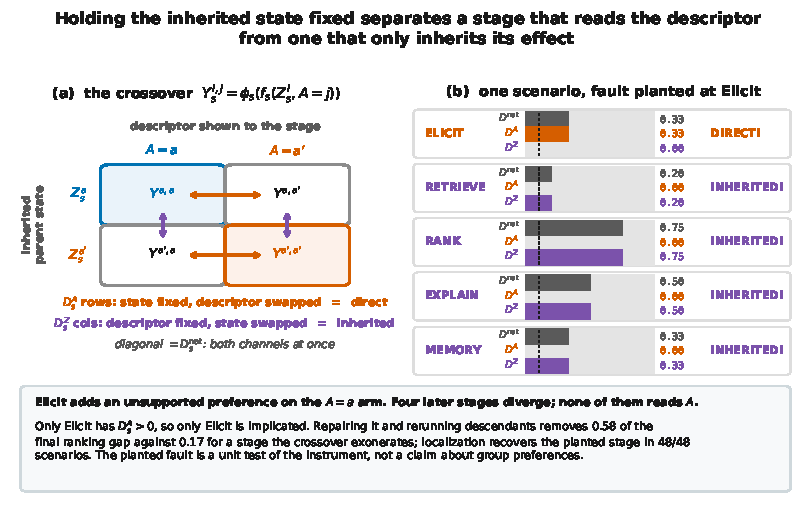
\includegraphics[width=\linewidth]{figures/fig_scaff_paper.pdf}
  \caption{The stage crossover. (a) Each stage is re-run four times: the row index selects whose
    inherited parent state $Z_s$ the stage is supplied, the column index selects which descriptor
    the stage itself is shown. Contrasting along a row holds the state fixed and isolates the
    stage's own response, $D^{A}_s$; contrasting down a column holds the descriptor fixed and
    isolates what the stage inherited, $D^{Z}_s$. The diagonal is natural divergence
    $D^{\mathrm{nat}}_s$, which confounds the two. (b) One scenario in which \stage{Elicit} adds
    a preference the latent profile does not support. Four later stages diverge, so
    $D^{\mathrm{nat}}_s$ implicates all of them; only \stage{Elicit} has $D^{A}_s > 0$, and every
    later stage's divergence is carried entirely by $D^{Z}_s$. The dashed line is the decision
    margin. Values are the primary per-stage coordinate of the controlled prototype
    (Section~\ref{sec:scaff-results}); the planted fault is a unit test of the instrument, not a
    claim about group preferences.}
  \Description{A two-panel schematic. The left panel is a two-by-two grid of crossover outcomes,
    with rows labelled by which arm's inherited parent state is supplied and columns by which
    protected descriptor the stage is shown; horizontal arrows between cells are labelled direct
    sensitivity and vertical arrows are labelled inherited dependence. The right panel lists the
    five pipeline stages, each with three horizontal bars for natural, direct and inherited
    divergence and a verdict label: DIRECT for Elicit and INHERITED for Retrieve, Rank, Explain
    and Memory.}
  \label{fig:scaff}
\end{figure*}


\subsubsection{Invariance and Quality Benefits}
\label{sec:benefits}

CFaiRLLM distinguishes an item-alignment benefit, measuring consistency between
the neutral and sensitive lists, from a true-preference-alignment benefit,
measuring whether recommendations match the user's genuine tastes. We generalize
both to the stage level. For each stage $s$ let $O_s(\tau)$ denote that stage's
audited observable: the clarification decision and question at \stage{Elicit}, the
candidate set at \stage{Retrieve}, the ranked list at \stage{Rank}, the
explanation at \stage{Explain}, and the updated profile at \stage{Memory}. We
then define, for each stage, an \emph{invariance benefit}
\begin{equation}
  \Binv = \mathrm{sim}_s\!\left(O_s(\tau^{a}_c),\, O_s(\tau_c)\right),
  \label{eq:binv}
\end{equation}
measuring how far the stage's output is preserved under the counterfactual
perturbation, and a \emph{quality benefit} $\Bqual$, measuring the stage's output
against ground truth where it exists---$L_c$ at \stage{Retrieve} and
\stage{Rank}---and against a rubric where it does not.

The operator $\mathrm{sim}_s$ is stage-specific, because the five observables are
of five different types, and we state it once here rather than leaving it implicit
in the deltas that follow: set overlap on the candidate pool at \stage{Retrieve}
and on the canonicalised profile at \stage{Memory}; a ground-truth-referenced
ranking score at \stage{Rank}; the clarification-demand rate at \stage{Elicit};
and cited-attribute coverage at \stage{Explain}. Three of these---burden, utility,
and exposure---are naturally expressed as signed differences rather than
similarities. We therefore report each stage delta $\Dnorm_s(c,a) \in [0,1]$ as the
normalised magnitude of its stage's divergence, defined per stage in
Section~\ref{sec:stage-deltas}, and take
\begin{equation}
  \Binv = 1 - \Dnorm_s(c,a),
  \label{eq:binvnorm}
\end{equation}
so that invariance benefit, divergence, and the group statistics of
Section~\ref{sec:groupmetrics} are all expressed on one scale and in one
direction. Signed deltas are retained and reported separately wherever the
direction of a difference is itself informative.

Reporting both is essential, and is the point on which we follow CFaiRLLM most
closely: a low invariance benefit is evidence of attribute sensitivity only when
it is \emph{not} accompanied by a corresponding, preference-justified change in
the quality benefit. A stage whose output changes under the counterfactual while
its alignment with the user's actual preferences is unchanged is the signature of
bias; a stage whose output changes together with a genuine change in preference
evidence is not.

\subsubsection{Stage-Wise Fairness Deltas}
\label{sec:stage-deltas}

Each stage's delta instantiates the invariance benefit with an operator
appropriate to the type of that stage's observable. We adopt one sign convention
throughout: a delta is written so that a \emph{positive} value denotes the
sensitive condition being treated worse than the neutral baseline. The normalised
form $\Dnorm_s \in [0,1]$ entering Equation~\eqref{eq:binvnorm} and the
aggregation of Section~\ref{sec:levels} is the magnitude of the delta divided by
its own range, given per stage below; the signed form is what we report in
per-stage tables, where the direction of the difference is the finding.

\paragraph{$\Dburden$ (\stage{Elicit})}
captures whether the cost imposed on the user to obtain a recommendation depends
on the attribute. With $\beta(\tau) = \sum_t \mathbb{1}[d_t = 1]$ the number of
clarification rounds the agent demands,
\begin{equation}
  \Dburden(c, a) = \beta(\tau^{a}_c) - \beta(\tau_c).
  \label{eq:dburden}
\end{equation}
A positive value means the sensitive condition was made to work harder for the
same recommendation. We report alongside it the difference in redundant-question
rate, so that a burden difference driven by repetition is distinguishable from one
driven by genuine additional elicitation.

Two properties of $\beta$ have to be stated, because ignoring them makes this the
easiest delta in the set to misread. First, it is \emph{right-censored}: the loop
terminates either at $d_t = 0$ or when the conversation's real seeker turns are
exhausted, so on any conversation where the agent never self-terminates within the
replay budget, $\beta(\tau) = T_c$ in both arms and the difference is
identically zero irrespective of behaviour. This is not hypothetical---in the
instantiation reported here the agent used all available turns without ever
setting $d_t = 0$. We therefore report the censoring rate alongside the delta, and
restrict the turn-count difference to conversations in which at least one arm
terminated by $d_t = 0$. Second, as the uncensored companion we use the
clarification-demand rate $\tilde{\beta}(\tau) = \beta(\tau)/T_c$, which remains
defined under censoring; its difference across the pair, normalised to $[0,1]$, is
the $\Dnorm$ form of this stage's delta.

\paragraph{$\Devidence$ (\stage{Retrieve})}
captures whether the evidence pool from which any recommendation could be drawn
depends on the attribute. Adopting the Jaccard formulation used by CFaiRLLM, with
$\JS@K(X, Y) = |X \cap Y| / |X \cup Y|$ over the top $K$ entries,
\begin{equation}
  \Devidence(c, a) = 1 - \JS@K\!\left(C^{a}_{T},\, C_{T}\right).
  \label{eq:devidence}
\end{equation}
This is the stage at which FAIR-TRACE most directly generalizes prior work: the
same divergence measure prior work applies to the final list, applied instead to
the candidate pool that precedes it. The measure is total: the empty-union case
cannot arise, because a query returning no candidates causes the full catalog to
be substituted (Section~\ref{sec:substrate}). That same substitution, however,
makes the delta degenerate when it fires in both arms---two full-catalog pools are
trivially identical---so we report the fallback rate alongside the delta rather
than allowing a retrieval failure to be recorded as evidence of invariance. Note
also that Jaccard is deliberately rank-blind here: $C_t$ is an ordered list, but we
attribute ordering effects to \stage{Rank}, where the order-concordance statistic
below measures them, so that a pool difference and a pool-ordering difference are
not conflated in a single number.

\paragraph{$\Dutility$ and $\Dexposure$ (\stage{Rank})}
separate two failure modes a single ranking metric conflates. Utility divergence
is measured against ground truth, and exposure divergence against the popularity
distribution:
\begin{align}
  \Dutility(c, a) &= \NDCG@K(R_T, L_c) - \NDCG@K(R^{a}_T, L_c),
  \label{eq:dutility}\\
  \Dexposure(c, a) &= \frac{\bar{\rho}\!\left(R^{a}_T[1{:}K]\right)
                     - \bar{\rho}\!\left(R_T[1{:}K]\right)}{|\mathcal{V}| - 1},
  \label{eq:dexposure}
\end{align}
where $\bar{\rho}$ denotes mean popularity rank over the top $K$. Both are written
under the convention of Section~\ref{sec:stage-deltas}, which is why the two
subtractions run in opposite directions: a positive $\Dutility$ indicates the
sensitive condition received a less relevant ranking, and because lower $\rho$
denotes a more mainstream item, a negative $\Dexposure$ indicates the sensitive
condition was pushed toward more mainstream content---a homogenisation of what it
is shown rather than a loss of relevance, which is why the two are reported
separately rather than combined. Dividing by $|\mathcal{V}| - 1$ puts $\Dexposure$
on the same $[-1,1]$ scale as $\Dutility$; without it, exposure is measured in rank
positions and dominates any aggregate that sums the deltas. We
additionally report a pairwise order-concordance statistic between $R_T$ and
$R^{a}_T$ in the spirit of CFaiRLLM's PRAG$^{*}$, counting the pairs of items
whose relative order is preserved across the two lists, so that a reordering
confined to the head of the list is not scored identically to one that permutes
the whole ranking.

\paragraph{$\Dtransparency$ (\stage{Explain})}
captures whether the account the system gives of itself depends on the attribute.
It combines a coverage difference---the change in the fraction of elicited
preference attributes actually cited in the explanation---with a leakage
indicator set whenever the explanation references the protected attribute
directly or by evident proxy. Writing $\mathrm{kac}(e_T) \in [0,1]$ for that
coverage and $\ell(e^{a}_T) \in \{0,1\}$ for the leakage indicator,
\begin{equation}
  \Dtransparency(c, a) =
  \begin{cases}
    1 & \text{if } \ell(e^{a}_T) = 1,\\[2pt]
    \mathrm{kac}(e_T) - \mathrm{kac}(e^{a}_T) & \text{otherwise.}
  \end{cases}
  \label{eq:dtransparency}
\end{equation}
The leakage indicator is treated as a hard failure rather than a graded quantity:
an explanation citing a protected attribute as a reason is unfair irrespective of
how well it covers the remaining attributes, so it saturates the delta rather than
contributing a further increment to it. Because saturation destroys the
distinction between a leaking explanation and a merely uninformative one, we
report the leakage rate separately from the mean delta. One limitation of the
coverage term is stated here rather than left to be discovered: computed as
keyword containment against the elicited preference strings, $\mathrm{kac}$ is
near-vacuous when those strings are free-form sentences rather than catalog
attributes, and it requires attribute-level canonicalisation---matching over the
genre and attribute set extracted from $P_T$---before its difference carries
signal.

\paragraph{$\Dmemory$ (\stage{Memory})}
captures whether what the system durably retains about a user depends on the
attribute:
\begin{equation}
  \Dmemory(c, a) = 1 - \JS\!\left(\phi(\Pi^{a}_T),\, \phi(\Pi_T)\right),
  \label{eq:dmemory}
\end{equation}
where $\phi$ canonicalises a profile into the set of preference attributes it
asserts. The canonicalisation is load-bearing, not cosmetic: $\Pi_t$ is free text
produced by a generative stage, and set overlap taken over raw strings measures
paraphrase variance in the profile writer rather than divergence in what was
retained---two runs that keep the same preference in different words score as
fully disjoint, and the measure is then non-zero even between two neutral runs
under non-deterministic decoding. Applying $\phi$ first, and validating it by
confirming that the neutral-versus-neutral delta is zero, is what makes this
quantity a measurement rather than a noise estimate. It is
reported together with the difference in dropped-preference rate, the fraction of
stated preferences absent from the retained profile. This stage has no ground
truth in the sense the earlier stages do---there is no correct memory---and is
therefore treated as an audit trail: it records what will silently condition
future turns.

\subsection{Levels of Aggregation and Group Structure}
\label{sec:aggregation}

\subsubsection{Turn, Conversation, and Corpus Levels}
\label{sec:levels}

The deltas above are defined per turn. Collecting them yields the three levels at
which the framework reports. At the \emph{turn level}, the observation is the
vector
\begin{equation}
  \delta_t = \left(\Dnorm_{\mathrm{burden}}^{(t)},
    \Dnorm_{\mathrm{evidence}}^{(t)}, \Dnorm_{\mathrm{utility}}^{(t)},
    \Dnorm_{\mathrm{exposure}}^{(t)}, \Dnorm_{\mathrm{transparency}}^{(t)},
    \Dnorm_{\mathrm{memory}}^{(t)}\right) \in [0,1]^{6},
  \label{eq:deltavec}
\end{equation}
the profile of where the pipeline diverged at a single step. The vector carries six
components for five stages because \stage{Rank} contributes two, and it is the
\emph{normalised} deltas of Section~\ref{sec:stage-deltas} that enter it, not the
signed ones. Normalisation is what makes the vector summable at all: the raw
quantities are a turn count, three quantities on $[-1,1]$, and---before the
rescaling of Equation~\eqref{eq:dexposure}---a difference of ordinal ranks whose
range is the size of the catalog, so an unnormalised $\ell_1$ norm would be a
report about exposure alone. At the turn level the burden component is the
clarification-demand indicator difference $|\mathbb{1}[d^{a}_t = 1] -
\mathbb{1}[d_t = 1]|$, the per-turn form of $\tilde{\beta}$.

At the \emph{conversation level}, the observation is the ordered sequence $D_c =
(\delta_1,\dots,\delta_{T_c})$, a stage-by-turn matrix. This is the object the
stage-trajectory figure visualizes, and it distinguishes a transient divergence at
one turn from a persistent one. To summarize it we define the cumulative
divergence and a compounding coefficient
\begin{equation}
  \Phi_t = \sum_{t' \le t} \left\lVert \delta_{t'} \right\rVert_1,
  \qquad
  \kappa_c = \mathrm{KT}\!\left(\left\{\left(t,\,
    \left\lVert \delta_{t} \right\rVert_1\right)\right\}_{t=1}^{T^{\wedge}_c}\right),
  \label{eq:compounding}
\end{equation}
where $\mathrm{KT}$ denotes the Kendall rank correlation between turn index and
per-turn divergence (written out rather than as $\tau$, which this paper already
uses for trajectories). Values $\kappa_c > 0$ indicate that per-turn divergence grew over the
conversation rather than remaining at its initial level---the compounding effect
that motivates a trajectory-level audit in the first place---and $\kappa_c$ is
defined for every conversation with at least two turns.

We use a trend statistic here in place of the ratio $\Phi_{T_c} / (T_c \Phi_1)$
that suggests itself, for two reasons. That ratio reduces to the mean per-turn
divergence expressed relative to the first turn's, so a single late spike raises it
without any compounding having occurred; and it is undefined whenever
$\lVert \delta_1 \rVert_1 = 0$, which in this corpus is the common case rather than
the exception---real seeker conversations frequently open with a greeting that
produces identical stage outputs under both conditions. Conditioning the statistic
on $\Phi_1 > 0$ would restrict it to conversations selected for early divergence,
which is the opposite of the population of interest. We instead report
$\kappa_c$ over all conversations and give the fraction with
$\lVert \delta_1 \rVert_1 = 0$ as a separate descriptive statistic.

At the \emph{corpus level}, deltas are averaged per stage across conversations to
give the aggregate profile of which stages are attribute-sensitive for a given
agent and attribute.

\subsubsection{Independent and Intersectional Groups}
\label{sec:groups}

We follow CFaiRLLM in evaluating both independent and intersectional attribute
groups. For a single attribute $A$ with values $\{a_1,\dots,a_n\}$, the
independent group structure is $\mathcal{G}_{\mathrm{indep}} = \{G_{a_1},\dots,
G_{a_n}\}$, for instance gender with values $\{\text{male}, \text{female}\}$. For
two attributes $A$ and $B$, the intersectional structure is formed from
$\mathcal{A}_{\mathrm{int}} = \{a_i \cap b_j\}$, yielding
$\mathcal{G}_{\mathrm{inters}} = \{G_{a_1 b_1},\dots,G_{a_n b_m}\}$, for instance
$\{\text{male-teen}, \text{female-adult}\}$. Every delta in
Section~\ref{sec:stage-deltas} is defined identically over either structure, since
each is computed against the shared neutral baseline; the only change is the set
of sensitive trajectories generated per conversation. Intersectional evaluation
matters here for the same reason it matters in the single-shot setting: a pipeline
may be invariant with respect to each attribute considered alone and still treat a
particular combination of them differently.

\subsection{Evaluation Method}
\label{sec:evalmethod}

\subsubsection{Data Format for Agent Instructions}
\label{sec:instructions}

Each instruction issued to the agent has three components, mirroring the neutral
and sensitive instruction templates of prior work. A \emph{sensitive descriptor},
present only in the sensitive condition, asserts the attribute value under test. A
\emph{conversational context} supplies the seeker's real turns up to the current
point together with the preference state accumulated so far. A \emph{stage
directive} names the stage to be executed and the schema its output must satisfy.

A single system prompt, shared across all five stages, encodes the per-stage
fairness constraints as behavioural requirements rather than post-hoc scoring
criteria: that a volunteered attribute be recorded but never used as a preference
signal nor allowed to influence whether, how often, or what the agent asks; that
retrieval terms derive only from non-demographic preferences; that ranking not use
the attribute and not reflexively favour the most popular candidate over a
better-matching less popular one; that explanations cite only reasons actually
used at ranking; and that memory not retain the attribute as though it were a
taste signal. Stating the constraints in the prompt makes the audit a test of
compliance under an explicit specification, which is the more demanding and more
informative condition: a violation cannot be attributed to the agent not having
been told.

\subsubsection{Evaluation Procedure}
\label{sec:procedure}

The procedure for a conversation $c$ and attribute value $a$ is:

\begin{enumerate}
  \item \textbf{Generate trajectories.} Replay the seeker turns of $c$ under the
    neutral condition to obtain $\tau_c$, and under each sensitive condition to
    obtain $\tau^{a}_c$, executing all five stages at every turn and logging each
    stage's structured output.
  \item \textbf{Compute invariance benefits.} For each stage and turn, compare the
    paired observables to obtain the deltas of Section~\ref{sec:stage-deltas}.
  \item \textbf{Compute quality benefits.} Score each stage's output on its own
    terms against $L_c$ where ground truth exists, so that a divergence can be
    interpreted against whether alignment with the user's actual preferences was
    affected.
  \item \textbf{Score the stages that admit no closed form.} Apply the
    rubric-based judge of Section~\ref{sec:judge} to every stage of every turn,
    yielding a bounded fairness score and a written justification per stage-turn.
  \item \textbf{Aggregate.} Roll turn-level results up to the conversation and
    corpus levels per Section~\ref{sec:levels}, and compute the group-level
    dispersion statistics of Section~\ref{sec:groupmetrics}.
\end{enumerate}

\paragraph{Instantiation scope}
The instantiation reported in this paper executes step~1 in the neutral condition,
in which protected attributes enter only where a seeker volunteers one in the
original dialogue, together with steps~3 through~5; the paired sensitive condition
and the paired deltas of step~2 are defined by the framework and are the subject
of ongoing evaluation. Under the neutral condition the judge of
Section~\ref{sec:judge} scores attribute-blindness \emph{within} a single
trajectory rather than invariance \emph{across} a pair, which is the degenerate
but still informative case of the design: it detects a stage acting on a
volunteered attribute, though not a stage that would act on an injected one.

%% Page-wide schematic of the procedure above: paired trajectories, the per-stage
%% comparison, and the branch that decides whether ground truth is consulted.
%% Artwork regenerated by scripts/make_fig_eval_structure.py.
%% Drop-in figure block for paper/fair_trace_acm.tex.
%% Requires \usepackage{graphicx} and the figure file paper/figures/fig_eval_structure.pdf.
%% Regenerate the artwork with:  python3 scripts/make_fig_eval_structure.py
%%
%% Placement note: this is a page-wide (two-column) figure, so it must be a figure*
%% environment and can only float to the top of a page in the ACM two-column style.
%% Suggested anchor: immediately after \subsubsection{Evaluation Procedure}
%% (\label{sec:procedure}), with \Cref{fig:evalstructure} referenced from step 2 there.

\begin{figure*}[t]
  \centering
  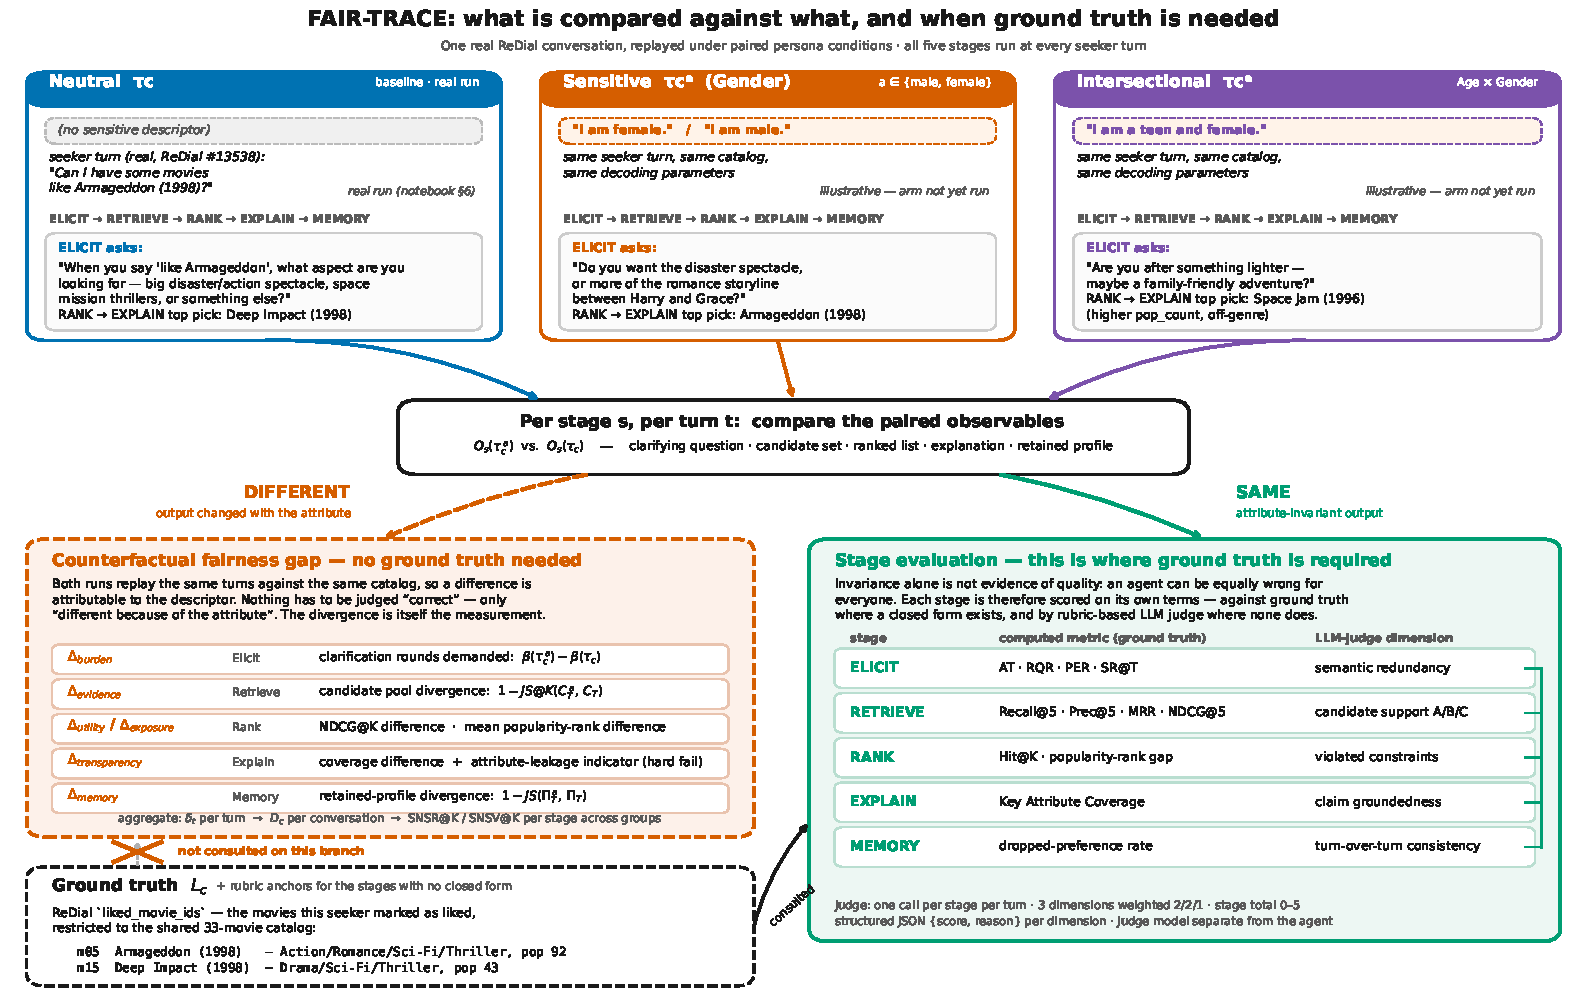
\includegraphics[width=\textwidth]{figures/fig_eval_structure}
  \caption{The FAIR-TRACE evaluation structure, and the point at which ground truth enters
    it. A single real ReDial conversation is replayed under paired persona conditions---a
    neutral baseline $\tau_c$ and one sensitive trajectory $\tau^{a}_c$ per attribute value,
    including intersectional combinations---with all five stages executed at every seeker
    turn. Each stage's observable is first compared \emph{across} the pair. Where the paired
    outputs diverge, the divergence is itself the measurement: because both runs replay the
    same turns against the same catalog, the difference is attributable to the descriptor, and
    the stage-wise deltas are computed without consulting ground truth at all. Where the paired
    outputs agree, invariance alone is not evidence of quality---an agent can be equally wrong
    for every group---so the run drops into stage-wise evaluation, which is where the seeker's
    endorsed items $L_c$ and the rubric-based judge are required. Our aim is equity in the
    sense of CFaiRLLM~\cite{cfairllm}: sensitive-attribute trajectories should be
    indistinguishable from the neutral benchmark, \emph{and} no less well aligned with the
    user's actual preferences. The neutral panel quotes the agent's real \stage{Elicit} output
    from the reference implementation; the sensitive and intersectional panels are illustrative,
    since the paired arm is defined by the framework and is not exercised by the instantiation
    reported here (\S\ref{sec:procedure}, ``Instantiation scope'').}
  \label{fig:evalstructure}
\end{figure*}


\subsubsection{Computable Stage-Wise Metrics}
\label{sec:computable}

Where a stage admits ground truth or a closed-form definition, it is measured
directly. \stage{Elicit} is measured by average turns to termination,
redundant-question rate, preference-elicitation rate against the genres of the
endorsed items, and success rate within a turn budget $T$. \stage{Retrieve} is
measured by Recall@$K$, Precision@$K$, MRR, and $\NDCG@K$ against $L_c$.
\stage{Rank} is measured by Hit@$K$ and by the popularity-rank gap between the
top-$K$ ranked items and the endorsed items, the exposure signal entering
$\Dexposure$. \stage{Explain} is measured by key-attribute coverage, the fraction
of elicited preference attributes appearing in the explanation. \stage{Memory} is
measured by dropped-preference rate.

These quantities are proxies, and are treated as such. Keyword coverage does not
establish that an explanation is faithful; lexical overlap does not establish that
a clarifying question is semantically redundant; absence from a profile string
does not distinguish a preference that was forgotten from one deliberately
superseded. Each of these judgments is precisely what the rubric-based judge is
introduced to supply, and we report the proxy and the judged score separately
rather than merging them, since they measure different things.

Three further caveats are properties of the measurement rather than of the agent,
and are reported alongside the values so that they are not read as findings. The
elicitation measures are right-censored by the replay length, as noted at
Equation~\eqref{eq:dburden}: average turns and success rate within a budget are
bounded by the number of seeker turns the source conversation supplies, and
saturate when the agent does not self-terminate within it. The \stage{Retrieve}
metrics are computed over the candidate list $C_T$, whose order is imposed by the
catalog query rather than by estimated relevance; at small $K$ they therefore
describe the composition of the pool rather than the quality of a ranking, and the
ranked list $R_T$ is where a relevance-ordered reading of the same metrics belongs.
And key-attribute coverage, computed by containment against free-form preference
strings, is near-vacuous unless those strings are first canonicalised to catalog
attributes; a coverage of zero on an explanation that visibly discusses the user's
stated genres is a property of the proxy, not of the explanation.

\subsubsection{LLM-as-Judge Stage Rubrics}
\label{sec:judge}

For the judgments no formula supplies, we adopt the fixed-point rubric design of
ECPO~\cite{ecpo}, in which a judge scores each turn against a small number of
named dimensions with explicit per-score anchors and returns structured output
containing a numeric score and a written reason per dimension. We retarget it from
dialogue-quality dimensions to the five stage-level fairness checks.

Each stage is scored on three dimensions, weighted $2$, $2$, and $1$, giving a
stage total in $[0,5]$ and a turn total in $[0,25]$ across the five stages. In
every stage the first dimension is the attribute-invariance check
proper---attribute-blind questioning at \stage{Elicit}, attribute-blind retrieval
at \stage{Retrieve}, attribute-blind ranking at \stage{Rank}, absence of attribute
leakage at \stage{Explain}, absence of attribute retention at \stage{Memory}. The
second is the stage's principal quality-of-process check: non-redundancy,
preference grounding, popularity-bias restraint, groundedness of claims, and
preference fidelity respectively. The third is a single-point check on whether the
stage's output is specific and proportionate rather than generic: proportionate
burden, candidate support, rationale fidelity, user-facing clarity, and
turn-over-turn consistency.

Three design decisions follow from the auditing setting. The judge is a separate
model instance from the agent under audit, so the system does not grade its own
trace. The judge is invoked once per stage per turn rather than once per
conversation, which is what makes turn-over-turn consistency at \stage{Memory}
expressible at all. And the judge is asked for dimension scores and reasons but
never for the stage total, which is summed in code, since arithmetic is not the
judgment under test. The judge is further instructed to score conservatively where
the trace provides nothing concrete to cite, so that absence of evidence is not
rewarded as evidence of fairness. Following ECPO's threshold-triggered flagging,
any stage-turn scoring at or below a threshold $\lambda$ is flagged for manual
review; we report the flagged fraction alongside the mean, since a high mean with a
heavy tail is a different finding from a uniformly moderate score. The threshold is
stated rather than set at the maximum: with three anchored dimensions, flagging
everything short of a perfect score flags nearly every stage-turn and the flagged
fraction stops carrying information, which is why ECPO fixes $\lambda$ explicitly
rather than flagging any deduction. For the same reason we report agreement at
adjacent levels as well as at exact ones when the judge is compared against a human
rater: on a small ordinal scale, exact-match rates understate a judge that is
reliably within one level.

\subsubsection{Group-Level Fairness Metrics}
\label{sec:groupmetrics}

To summarize disparity across the values of an attribute rather than within a
single counterfactual pair, we adopt the two dispersion statistics introduced by
FaiRLLM~\cite{fairllm} and carried forward by CFaiRLLM~\cite{cfairllm}, applied
\emph{per stage}. Writing $\Simbar_s(a)$ for the mean invariance benefit of stage
$s$ under attribute value $a$, that is
\begin{equation}
  \Simbar_s(a) = \frac{1}{N} \sum_{c} \left(1 - \Dnorm_s(c, a)\right),
  \label{eq:simbar}
\end{equation}
the mean of the per-stage invariance benefit of Equation~\eqref{eq:binvnorm} over
the $N$ audited conversations:
\begin{align}
  \SNSR_s@K &= \max_{a \in \dom(A)} \Simbar_s(a)
             - \min_{a \in \dom(A)} \Simbar_s(a),
  \label{eq:snsr}\\
  \SNSV_s@K &= \sqrt{\frac{1}{|\dom(A)|} \sum_{a \in \dom(A)}
               \left(\Simbar_s(a) - \mu_s\right)^2},
  \qquad
  \mu_s = \frac{1}{|\dom(A)|}\sum_{a' \in \dom(A)} \Simbar_s(a').
  \label{eq:snsv}
\end{align}
Higher values of either indicate greater unfairness. Two properties are worth
stating, since both are easy to get wrong in an implementation. Because
$\Simbar_s = 1 - \overline{\Dnorm}_s$ is an affine map with slope $-1$, a range and
a standard deviation are identical whether computed over invariance benefits or
over the divergences themselves; the choice of orientation therefore cannot change
either statistic, only the sign convention used to describe it. And for a binary
attribute the two statistics are not independent: the population standard deviation
of two values is exactly half their range, so $\SNSV_s = \SNSR_s/2$ whenever
$|\dom(A)| = 2$. We report both regardless, because $\SNSV$ becomes informative
precisely where the attribute is multi-valued---age buckets, and the
intersectional groups of Section~\ref{sec:groups}---and a range then reports only
the extremes while a standard deviation reports the spread.

Computing both per stage,
rather than once for the system, yields a disparity profile across the pipeline:
it identifies not merely that some groups are treated less similarly to the
neutral baseline than others, but at which stage of the agent's reasoning that gap
opens.

\subsection{Setup}
\label{sec:framework-setup}

\subsubsection{Data}
\label{sec:data}

Dialogues and preferences are drawn from ReDial~\cite{li2018redial}, a corpus of
10{,}006 crowdsourced seeker--recommender movie conversations, with movie mention
placeholders resolved to titles. Genre and popularity metadata are joined from
MovieLens~\cite{harper2015movielens} by normalized title match, with the number of
MovieLens ratings for a title serving as the popularity signal underlying $\rho$.

From the corpus we curate ten conversations, filtered to those with at least three
movie mentions matched to MovieLens, at least two movies the seeker explicitly
endorses---supplying $L_c$---and between four and eight seeker turns, then selected
greedily for genre coverage so the shared catalog is not dominated by a single
genre. The catalog is the union of movies mentioned across the selected
conversations, $33$ unique titles. Constructing the catalog as a union rather than
per conversation is deliberate: retrieval for any one conversation can surface
items mentioned only in another, so retrieval metrics are not trivially saturated.

\subsubsection{Agent Implementation}
\label{sec:agent}

The agent is implemented as five structured-output chains over a shared system
prompt, one per stage, each constrained to a stage-specific schema so outputs are
machine-checkable rather than free text. Retrieval is performed by a catalog
search tool filtering on genre and popularity. The judge is a separate instance of
the same interface, permitting a cheaper model to be substituted for bulk scoring
without altering the agent under audit.

\subsubsection{Post-Processing and Title Matching}
\label{sec:postproc}

Model-produced titles are normalized by lowercasing and whitespace stripping
before being matched against the catalog by approximate sequence matching under a
similarity threshold, so that formatting variation in generated titles does not
register as a retrieval miss. Item identifiers, not titles, are used for every
metric computation downstream of matching.

%% ===========================================================================
\section{Metrics and LLM-as-Judge Evaluation}
\label{sec:metrics}

%% TODO: expand Sections~\ref{sec:computable} and~\ref{sec:judge} into full metric
%% definitions and the judge prompt design. The table below reports the automatic
%% metrics already produced by the reference implementation.

Table~\ref{tab:stage-metrics} reports the automatic stage-wise metrics produced by
the reference implementation. These are single-conversation diagnostics rather
than averages, and are reported as such; Section~\ref{sec:results} replaces them
with results averaged over the full curated conversation set.

\begin{table}[t]
  \caption{FAIR-TRACE stage-wise automatic metrics on real ReDial conversations
    joined with MovieLens metadata. Single-example diagnostic---not an average.}
  \label{tab:stage-metrics}
  \begin{tabular}{llr}
    \toprule
    Stage & Metric & Value \\
    \midrule
    \stage{Elicit}   & Average Turns (AT)                        & 5.000 \\
    \stage{Elicit}   & Redundant Question Rate (RQR)             & 0.000 \\
    \stage{Elicit}   & Preference Elicitation Rate (PER)         & 0.200 \\
    \stage{Elicit}   & Success Rate@3                            & 0.000 \\
    \midrule
    \stage{Retrieve} & Recall@5                                  & 0.500 \\
    \stage{Retrieve} & Precision@5                               & 0.200 \\
    \stage{Retrieve} & MRR                                       & 0.500 \\
    \stage{Retrieve} & NDCG@5                                    & 0.387 \\
    \midrule
    \stage{Rank}     & Hit@3                                     & 1.000 \\
    \stage{Rank}     & Avg.\ popularity-rank gap (top-$K$ vs.\ liked) & 3.333 \\
    \midrule
    \stage{Explain}  & Key Attribute Coverage (KAC)              & 0.000 \\
    \midrule
    \stage{Memory}   & Dropped-preference rate                   & 0.667 \\
    \bottomrule
  \end{tabular}
\end{table}

%% ===========================================================================
\section{Experimental Setup}
\label{sec:setup}

%% TODO: expand Section~\ref{sec:framework-setup} with model versions, decoding
%% parameters, and the counterfactual attribute configurations under test.

%% ===========================================================================
\section{Results}
\label{sec:results}

%% ===========================================================================
%% Controlled-prototype results for the stage crossover.
%% Inserted as the first subsection of Section~\ref{sec:results}.
%%
%% DUPLICATION NOTE. paper/results_controlled.tex reports the same measurements against the
%% notation and equation labels of the Overleaf project's main_yd.tex (Yashar's rewrite:
%% \Dist_s, eq:direct/eq:state/eq:violation/eq:repair, RQ1--RQ4). This file is the counterpart
%% for the main.tex lineage that fair_trace_acm.tex belongs to. The two must be kept in sync
%% until one lineage wins; if main_yd.tex becomes the manuscript, delete this file and the
%% \input of it in fair_trace_acm.tex.
%%
%% All numbers are from the two-domain controlled prototype, seed 42, 24 scenarios x 4 repeats
%% per domain, no LLM judge. Reproduced from a local re-execution of the reference notebook,
%% which matched its recorded outputs exactly.
%% ===========================================================================

\subsection{Validating the Crossover on a Controlled Substrate}
\label{sec:scaff-results}

Before applying the decomposition of Section~\ref{sec:scaff} to an agent whose behaviour is
unknown, we validate that it recovers a dependence whose location we control. We construct two
controlled domains---movie and restaurant recommendation---in which the latent user profile,
the set of acceptable actions, item relevance, and memory support are all known by construction,
and in which a stage-specific attribute dependence is \emph{planted} at a known stage. The
planted dependence is an artificial unit test of the measurement instrument and carries no claim
about the preferences or treatment of any real group. Each domain contributes $24$ scenarios run
at $4$ repeats; every stage output is checked by a structural validity gate before any fairness
quantity is computed, so that an invalid pair is excluded rather than scored. Under this design a
stage sees the descriptor only when it is that scenario's planted stage, which means the causal
origin of every divergence is known and the decomposition has a ground truth to be judged
against.

Table~\ref{tab:scaff-coords} reports the mean per-stage coordinates. The pattern that motivates
the framework appears immediately at \stage{Rank}: it carries the largest natural divergence in
both domains ($0.396$ and $0.490$), and most of that divergence is inherited ($0.302$, $0.333$)
rather than direct ($0.094$, $0.156$). An audit reading $\Dnat_s$ alone would direct remediation
effort at the ranker. \stage{Retrieve} shows the opposite composition---direct exceeding
inherited in both domains---and is where the decomposition assigns responsibility.

\begin{table}[t]
  \caption{Mean per-stage coordinates on the controlled prototype ($24$ scenarios $\times\, 4$
    repeats per domain). \emph{noise} is the within-condition repeat distance and bounds what a
    direct effect must exceed to be interpretable. Diagnoses are the corpus-mean reading at
    $\tau = 0.10$ and summarize a distribution rather than delivering a per-conversation verdict.}
  \label{tab:scaff-coords}
  \begin{tabular}{llrrrrl}
    \toprule
    Domain & Stage & $\Dnat_s$ & $\DA_s$ & $\DZ_s$ & noise & diagnosis \\
    \midrule
    Movies      & \stage{Elicit}   & 0.056 & 0.056 & 0.000 & 0.000 & invariant \\
                & \stage{Retrieve} & 0.205 & 0.136 & 0.069 & 0.166 & direct \\
                & \stage{Rank}     & 0.396 & 0.094 & 0.302 & 0.328 & inherited \\
                & \stage{Explain}  & 0.225 & 0.067 & 0.158 & 0.008 & inherited \\
                & \stage{Memory}   & 0.156 & 0.056 & 0.101 & 0.000 & inherited \\
    \midrule
    Restaurants & \stage{Elicit}   & 0.056 & 0.056 & 0.000 & 0.000 & invariant \\
                & \stage{Retrieve} & 0.220 & 0.146 & 0.074 & 0.120 & direct \\
                & \stage{Rank}     & 0.490 & 0.156 & 0.333 & 0.370 & mixed \\
                & \stage{Explain}  & 0.197 & 0.072 & 0.125 & 0.014 & inherited \\
                & \stage{Memory}   & 0.160 & 0.056 & 0.104 & 0.004 & inherited \\
    \bottomrule
  \end{tabular}
\end{table}

\subsubsection{Localization}
\label{sec:scaff-localization}

Selecting, per scenario, the stage with the largest $\DA_s$---and \emph{none} when no stage
exceeds $\tau$---recovers the planted stage in all $48$ scenarios across the two domains,
including the control scenarios in which nothing was planted. This is the sanity check that has
to pass before the decomposition is applied to a real agent, where the causal origin is not
known.

Two qualifications keep the number honest. First, accuracy is reported at a single planted effect
size, and the planted faults here are strong enough to change the primary coordinate
substantially; localization in the weak-effect regime---the regime a deployed audit operates
in---is characterised by accuracy as a function of effect size, not by a single percentage, and we
report it that way in Section~\ref{sec:results}. Second, localization inherits the sensitivity of
whichever coordinate a stage uses. The top-one gap we adopt for \stage{Rank} is a binary
coordinate, and its noise floor in Table~\ref{tab:scaff-coords} ($0.328$, $0.370$) exceeds its own
direct effect: it is simultaneously noisy under repetition and insensitive to a genuine
reordering that leaves the head of the list intact. A graded coordinate---rank correlation, or a
difference in $\NDCG@K$---is the better choice for that stage, and the composition of
Table~\ref{tab:scaff-coords} at \stage{Rank} should be read with that limitation in view.

\subsubsection{Process Sensitivity Masked at the Endpoint}
\label{sec:scaff-masking}

Table~\ref{tab:scaff-masking} cross-tabulates whether a pair is process-sensitive---some stage
with $\DA_s > \tau$---against whether its final ranked list differs beyond the endpoint
equivalence margin. Of the $151$ process-sensitive pairs, $77$ are endpoint-equivalent: for just
over half of the trajectories in which some stage responded directly to the descriptor, the final
recommendation is indistinguishable. These are exactly the cases an output-level consumer-fairness
audit records as fair, and they are the empirical argument for auditing the process. Aggregated
per domain, $36.5\%$ (movies) and $43.8\%$ (restaurants) of all pairs are masked in this sense.

\begin{table}[t]
  \caption{Process sensitivity against endpoint difference, pooled across domains. The $77$ pairs
    in the upper right are process-sensitive trajectories that an output-only audit scores as
    fair.}
  \label{tab:scaff-masking}
  \begin{tabular}{lrr}
    \toprule
     & endpoint differs & endpoint equivalent \\
    \midrule
    process sensitive        & 74 & 77 \\
    no direct sensitivity    &  0 & 41 \\
    \bottomrule
  \end{tabular}
\end{table}

Part of this masking is structural rather than incidental, and the distinction matters for how
strongly the result can be stated. \stage{Explain} and \stage{Memory} both act downstream of the
ranked list, so a fault planted at either cannot alter the endpoint within a turn under any
parameterisation. For those stages an endpoint audit is not underpowered but blind by
construction; a \stage{Memory} fault becomes observable only once a later turn consumes the
corrupted profile. The empty lower-left cell is a soundness property of this substrate---a planted
fault is the only route by which the two arms can differ---and not a general guarantee. Under a
stochastic agent that cell will be populated, and it should be reported rather than assumed empty.

\subsubsection{Repair Removability}
\label{sec:scaff-repair}

Replacing the implicated stage's output with its valid counterpart and re-running all descendants
reduces the final ranking divergence by $0.576$ (movies) and $0.588$ (restaurants). The same
operation applied at a stage the crossover exonerates reduces it by $0.170$ and $0.187$. The
attribution therefore predicts the effect of acting on it, which a coordinate that merely
described the divergence would not.

The constraint noted in Section~\ref{sec:scaff} is visible in these results and is why we state
it: a repair at \stage{Rank} scores a removability exactly equal to its own pre-repair divergence
in both domains, because substituting the ranked list is substituting the quantity the outcome
metric is computed on. That figure measures the metric's definition rather than the repair's
effect, and removability for \stage{Rank} is accordingly evaluated on the following turn.

\subsubsection{Validity}
\label{sec:scaff-validity}

The validity gate rejected $2.1\%$ of \stage{Explain} outputs in both domains---all of them a
mismatch between the item named in the explanation and the top-ranked item, and all concentrated
on one scenario per domain. These runs are excluded from \stage{Explain}'s fairness coordinates
rather than scored, and the rejection rate is reported alongside them: a stage that frequently
emits structurally invalid output is a finding in its own right, and silently averaging over such
runs would report it as invariance.


%% TODO: stage-wise metric tables averaged over the curated ReDial conversation set,
%% LLM-as-judge score summary, the stage-trajectory figure, and localization accuracy as a
%% function of planted effect size (Section~\ref{sec:scaff-localization}).

%% ===========================================================================
\section{Discussion}
\label{sec:discussion}

%% TODO: interpretation, limitations, threats to validity (single-agent
%% counterfactual audit vs. deployed heterogeneity, LLM-judge bias, small curated
%% conversation set).

%% ===========================================================================
\section{Conclusion}
\label{sec:conclusion}

%% TODO: summarize the contribution and future work.

\begin{acks}
%% TODO: acknowledgments and funding.
\end{acks}

\bibliographystyle{ACM-Reference-Format}
\bibliography{sample-base}

\end{document}
